\documentclass[14pt]{extbook}
\usepackage{multicol, enumerate, enumitem, hyperref, color, soul, setspace, parskip, fancyhdr} %General Packages
\usepackage{amssymb, amsthm, amsmath, bbm, latexsym, units, mathtools} %Math Packages
\everymath{\displaystyle} %All math in Display Style
% Packages with additional options
\usepackage[headsep=0.5cm,headheight=12pt, left=1 in,right= 1 in,top= 1 in,bottom= 1 in]{geometry}
\usepackage[usenames,dvipsnames]{xcolor}
\usepackage{dashrule}  % Package to use the command below to create lines between items
\newcommand{\litem}[1]{\item#1\hspace*{-1cm}\rule{\textwidth}{0.4pt}}
\pagestyle{fancy}
\lhead{Progress Quiz 5}
\chead{}
\rhead{Version A}
\lfoot{9912-2038}
\cfoot{}
\rfoot{Spring 2021}
\begin{document}

\begin{enumerate}
\litem{
Factor the quadratic below. Then, choose the intervals that contain the constants in the form $(ax+b)(cx+d); b \leq d.$\[ 24x^{2} +2 x -15 \]\begin{enumerate}[label=\Alph*.]
\item \( a \in [7.8, 8.8], \hspace*{5mm} b \in [-4, -1], \hspace*{5mm} c \in [2.5, 3.7], \text{ and } \hspace*{5mm} d \in [2, 7] \)
\item \( a \in [3.28, 4.33], \hspace*{5mm} b \in [-4, -1], \hspace*{5mm} c \in [5.8, 7.9], \text{ and } \hspace*{5mm} d \in [2, 7] \)
\item \( a \in [1.55, 2.02], \hspace*{5mm} b \in [-4, -1], \hspace*{5mm} c \in [10.1, 14.4], \text{ and } \hspace*{5mm} d \in [2, 7] \)
\item \( a \in [0.05, 1.4], \hspace*{5mm} b \in [-18, -15], \hspace*{5mm} c \in [-2.2, 2], \text{ and } \hspace*{5mm} d \in [14, 23] \)
\item \( \text{None of the above.} \)

\end{enumerate} }
\litem{
Factor the quadratic below. Then, choose the intervals that contain the constants in the form $(ax+b)(cx+d); b \leq d.$\[ 54x^{2} +15 x -25 \]\begin{enumerate}[label=\Alph*.]
\item \( a \in [8.3, 9.4], \hspace*{5mm} b \in [-8, 1], \hspace*{5mm} c \in [5.6, 6.32], \text{ and } \hspace*{5mm} d \in [2, 11] \)
\item \( a \in [3.1, 7.1], \hspace*{5mm} b \in [-8, 1], \hspace*{5mm} c \in [10.96, 12.37], \text{ and } \hspace*{5mm} d \in [2, 11] \)
\item \( a \in [25.8, 27.9], \hspace*{5mm} b \in [-8, 1], \hspace*{5mm} c \in [1.57, 3.31], \text{ and } \hspace*{5mm} d \in [2, 11] \)
\item \( a \in [0.1, 2.4], \hspace*{5mm} b \in [-31, -27], \hspace*{5mm} c \in [-0.38, 1.21], \text{ and } \hspace*{5mm} d \in [40, 48] \)
\item \( \text{None of the above.} \)

\end{enumerate} }
\litem{
Write the equation of the graph presented below in the form $f(x)=ax^2+bx+c$, assuming  $a=1$ or $a=-1$. Then, choose the intervals that $a, b,$ and $c$ belong to.
\begin{center}
    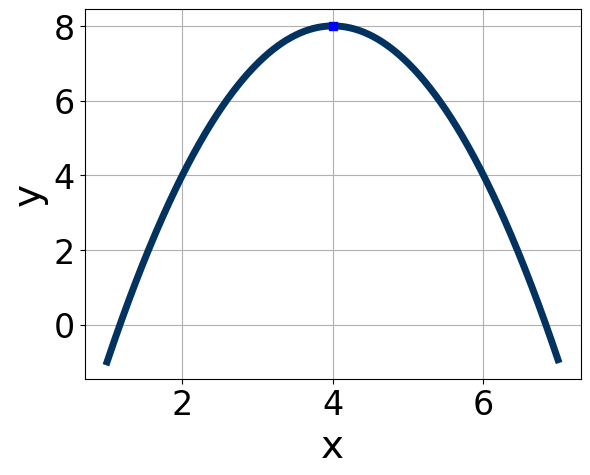
\includegraphics[width=0.5\textwidth]{../Figures/quadraticGraphToEquationA.png}
\end{center}
\begin{enumerate}[label=\Alph*.]
\item \( a \in [-3.1, 0], \hspace*{5mm} b \in [6, 10], \text{ and } \hspace*{5mm} c \in [-11, -5] \)
\item \( a \in [-3.1, 0], \hspace*{5mm} b \in [-12, -7], \text{ and } \hspace*{5mm} c \in [-25, -21] \)
\item \( a \in [-3.1, 0], \hspace*{5mm} b \in [-12, -7], \text{ and } \hspace*{5mm} c \in [-11, -5] \)
\item \( a \in [0.2, 1.9], \hspace*{5mm} b \in [-12, -7], \text{ and } \hspace*{5mm} c \in [24, 26] \)
\item \( a \in [0.2, 1.9], \hspace*{5mm} b \in [6, 10], \text{ and } \hspace*{5mm} c \in [24, 26] \)

\end{enumerate} }
\litem{
Graph the equation below.\[ f(x) = -(x-2)^2 - 14 \]\begin{enumerate}[label=\Alph*.]
\begin{multicols}{2}\item 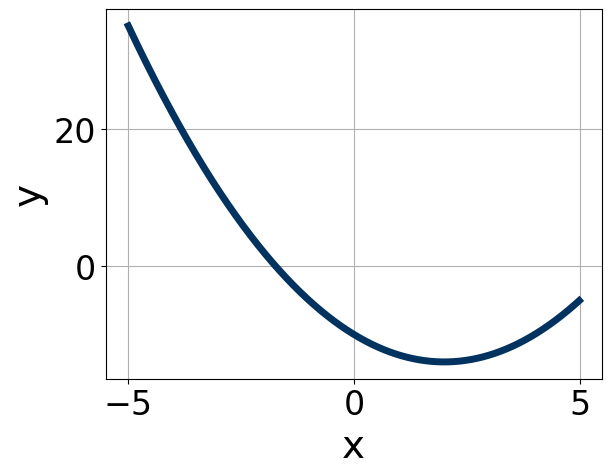
\includegraphics[width = 0.3\textwidth]{../Figures/quadraticEquationToGraphAA.png}\item 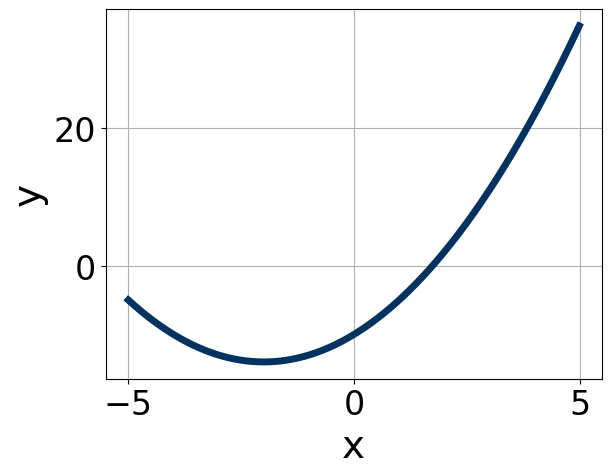
\includegraphics[width = 0.3\textwidth]{../Figures/quadraticEquationToGraphBA.png}\item 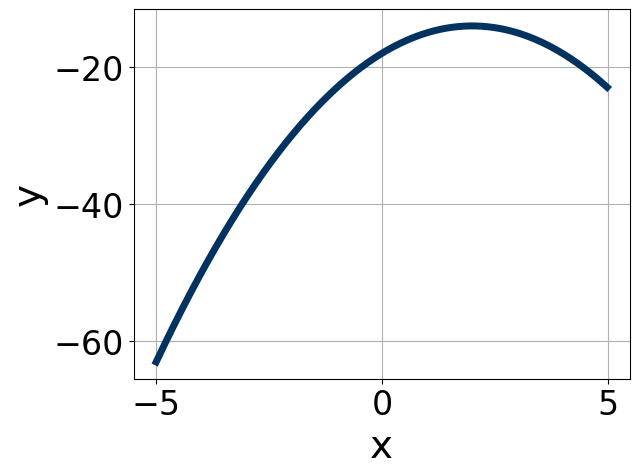
\includegraphics[width = 0.3\textwidth]{../Figures/quadraticEquationToGraphCA.png}\item 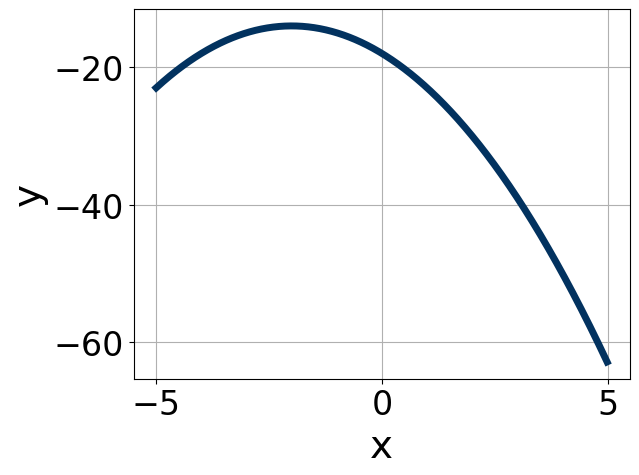
\includegraphics[width = 0.3\textwidth]{../Figures/quadraticEquationToGraphDA.png}\end{multicols}\item None of the above.
\end{enumerate} }
\litem{
Solve the quadratic equation below. Then, choose the intervals that the solutions $x_1$ and $x_2$ belong to, with $x_1 \leq x_2$.\[ 15x^{2} +32 x + 16 = 0 \]\begin{enumerate}[label=\Alph*.]
\item \( x_1 \in [-20.3, -19.79] \text{ and } x_2 \in [-12.02, -11.84] \)
\item \( x_1 \in [-1.46, -1.31] \text{ and } x_2 \in [-0.82, -0.68] \)
\item \( x_1 \in [-4.24, -3.96] \text{ and } x_2 \in [-0.38, -0.21] \)
\item \( x_1 \in [-2.83, -2.56] \text{ and } x_2 \in [-0.49, -0.34] \)
\item \( x_1 \in [-1.76, -1.55] \text{ and } x_2 \in [-0.78, -0.58] \)

\end{enumerate} }
\litem{
Solve the quadratic equation below. Then, choose the intervals that the solutions belong to, with $x_1 \leq x_2$ (if they exist).\[ 12x^{2} -15 x -4 = 0 \]\begin{enumerate}[label=\Alph*.]
\item \( x_1 \in [-19.98, -19.5] \text{ and } x_2 \in [19.5, 22.9] \)
\item \( x_1 \in [-3.11, -2.33] \text{ and } x_2 \in [16, 19.1] \)
\item \( x_1 \in [-0.35, 0.03] \text{ and } x_2 \in [0.4, 1.8] \)
\item \( x_1 \in [-1.73, -1.37] \text{ and } x_2 \in [-1.4, 1.4] \)
\item \( \text{There are no Real solutions.} \)

\end{enumerate} }
\litem{
Solve the quadratic equation below. Then, choose the intervals that the solutions $x_1$ and $x_2$ belong to, with $x_1 \leq x_2$.\[ 25x^{2} +60 x + 36 = 0 \]\begin{enumerate}[label=\Alph*.]
\item \( x_1 \in [-4.45, -3.23] \text{ and } x_2 \in [-0.52, -0.39] \)
\item \( x_1 \in [-6.7, -5.59] \text{ and } x_2 \in [-0.25, -0.08] \)
\item \( x_1 \in [-2.41, -1.99] \text{ and } x_2 \in [-0.76, -0.44] \)
\item \( x_1 \in [-1.24, 0.72] \text{ and } x_2 \in [-1.53, -0.9] \)
\item \( x_1 \in [-31.53, -29.59] \text{ and } x_2 \in [-30, -29.99] \)

\end{enumerate} }
\litem{
Write the equation of the graph presented below in the form $f(x)=ax^2+bx+c$, assuming  $a=1$ or $a=-1$. Then, choose the intervals that $a, b,$ and $c$ belong to.
\begin{center}
    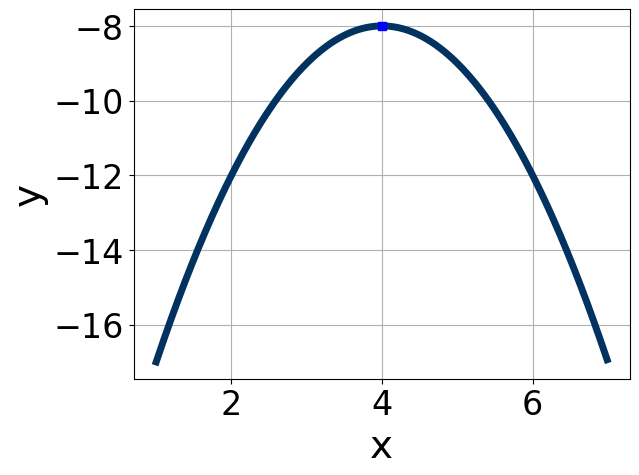
\includegraphics[width=0.5\textwidth]{../Figures/quadraticGraphToEquationCopyA.png}
\end{center}
\begin{enumerate}[label=\Alph*.]
\item \( a \in [0.7, 1.1], \hspace*{5mm} b \in [7, 9], \text{ and } \hspace*{5mm} c \in [8, 13] \)
\item \( a \in [-2.7, 0.8], \hspace*{5mm} b \in [7, 9], \text{ and } \hspace*{5mm} c \in [-28, -19] \)
\item \( a \in [-2.7, 0.8], \hspace*{5mm} b \in [-12, -7], \text{ and } \hspace*{5mm} c \in [-12, -5] \)
\item \( a \in [0.7, 1.1], \hspace*{5mm} b \in [-12, -7], \text{ and } \hspace*{5mm} c \in [8, 13] \)
\item \( a \in [-2.7, 0.8], \hspace*{5mm} b \in [-12, -7], \text{ and } \hspace*{5mm} c \in [-28, -19] \)

\end{enumerate} }
\litem{
Solve the quadratic equation below. Then, choose the intervals that the solutions belong to, with $x_1 \leq x_2$ (if they exist).\[ 13x^{2} -8 x -2 = 0 \]\begin{enumerate}[label=\Alph*.]
\item \( x_1 \in [-12.99, -12.6] \text{ and } x_2 \in [11.7, 14.3] \)
\item \( x_1 \in [-2.85, -2.45] \text{ and } x_2 \in [9.7, 11.8] \)
\item \( x_1 \in [-0.78, 0.4] \text{ and } x_2 \in [0.2, 2] \)
\item \( x_1 \in [-1.17, -0.43] \text{ and } x_2 \in [-0.4, 0.5] \)
\item \( \text{There are no Real solutions.} \)

\end{enumerate} }
\litem{
Graph the equation below.\[ f(x) = -(x+3)^2 + 15 \]\begin{enumerate}[label=\Alph*.]
\begin{multicols}{2}\item 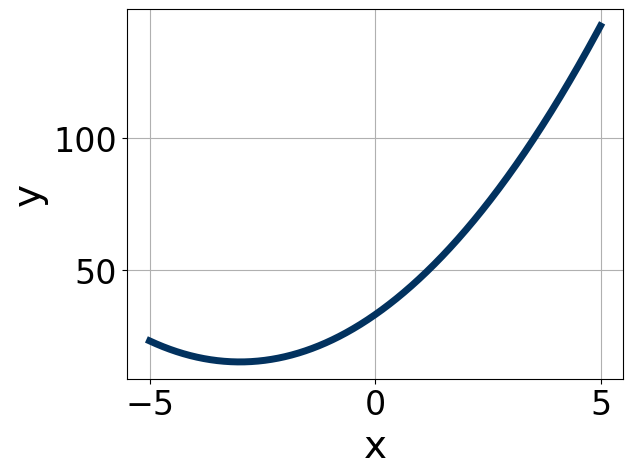
\includegraphics[width = 0.3\textwidth]{../Figures/quadraticEquationToGraphCopyAA.png}\item 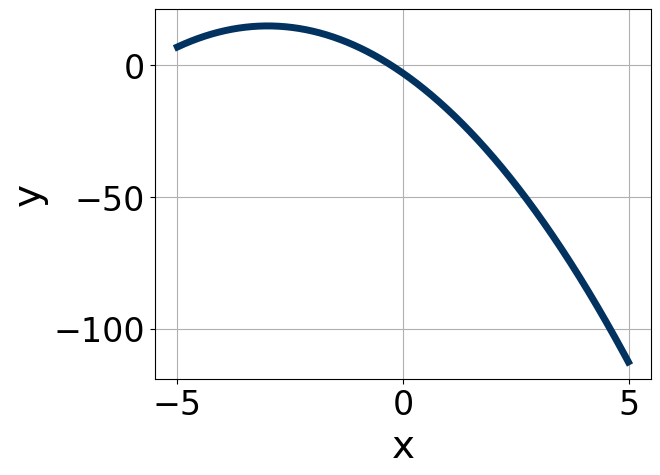
\includegraphics[width = 0.3\textwidth]{../Figures/quadraticEquationToGraphCopyBA.png}\item 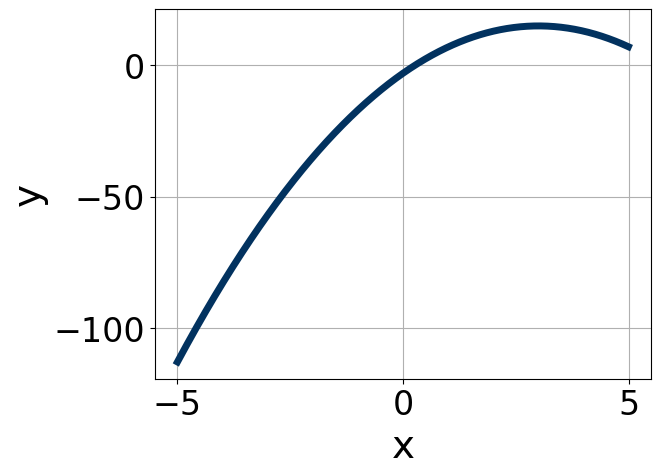
\includegraphics[width = 0.3\textwidth]{../Figures/quadraticEquationToGraphCopyCA.png}\item 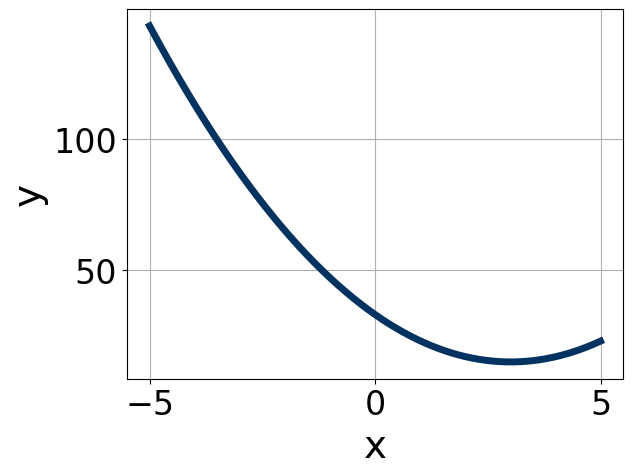
\includegraphics[width = 0.3\textwidth]{../Figures/quadraticEquationToGraphCopyDA.png}\end{multicols}\item None of the above.
\end{enumerate} }
\end{enumerate}

\end{document}